\documentclass[crop=false,10pt]{standalone}
\usepackage{standard}

\begin{document}
  \section{Learning} % (fold)
  \label{sec:Learning}
    \[
      \mathscr{S} \in V^s
      \separate
      \function{\mathscr{L}[\mathscr{S}]}{\setReal^{n\times m + n + m}}{\setReal}
      \separate
      \mathscr{L}[\mathscr{S}](ϑ) \define \frac{1}{s} \sum_{k=1}^s \ln p[ϑ]\roundBrackets{\mathscr{S}_k}
    \]
    \[
      \nabla_W \mathscr{L}[\mathscr{S}](ϑ) = \frac{1}{s} \sum_{k=1}^s \expect_ϑ\boxBrackets{\mathscr{V}\transpose{\mathscr{H}} \middle\vert \mathscr{S}_k} - \expect_ϑ\boxBrackets{\mathscr{V}\transpose{\mathscr{H}}}
    \]
    \begin{figure}
      \center
      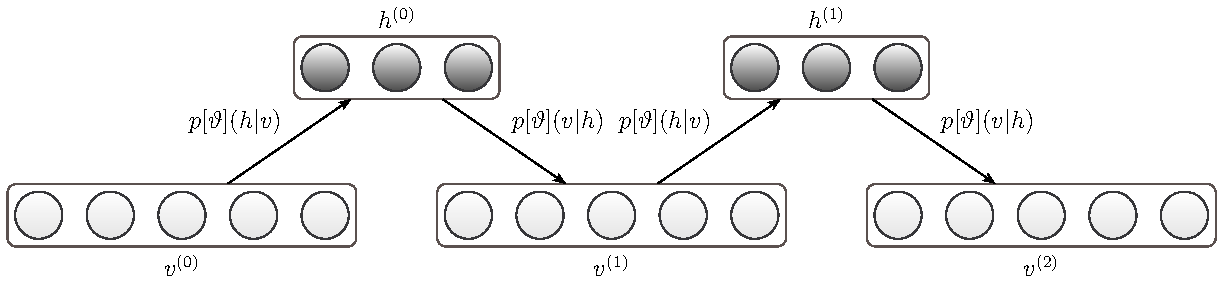
\includegraphics[width=0.9\textwidth]{figures/gibbs-sampling-scheme.pdf}
      \caption{%
        The figure shows the basic scheme of Gibbs sampling.
      }
      \label{fig:gibbs-sampling-scheme}
    \end{figure}
    \[
      \expect_ϑ\boxBrackets{\mathscr{V}\transpose{\mathscr{H}}} \approx v^{(k)}\transpose{h^{(k)}}
    \]
    \begin{figure}
      \center
      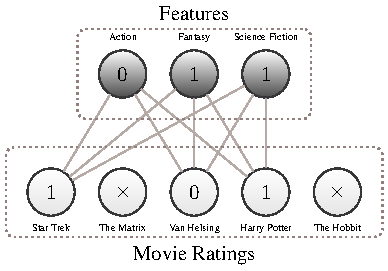
\includegraphics[width=0.9\textwidth]{figures/rbm-learning-example.pdf}
      \caption{%
        The figure shows the application of the learning algorithm to the movie ratings for some user.
      }
      \label{fig:gibbs-sampling-scheme}
    \end{figure}
  % section Learning (end)
\end{document}